\subsection{Interconnessione di componenti a due terminali}
\begin{figure}[H]
\centering
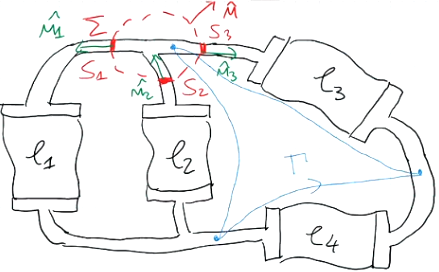
\includegraphics[width = 0.4\linewidth]{circuito_conduzione_stazionaria_nodo}
\end{figure}
\paragraph{LKC}
Si consideri una qualsiasi superficie chiusa $\Sigma$ che tagli tutti e soli i terminali
afferenti ad un nodo, tutte le superfici di questo tipo godono della proprietà di
equivalenza, si può costruire una classe di equivalenza ed applicare i risultati ottenuti
dallo studio della singola superficie a tutte le altre ad essa equivalenti.
Presa una superficie d'esempio si applica il principio di conservazione delle cariche:
$$
\oiint_\Sigma \vec{J}\cdot\hat{n}dS = 0\ \forall\ \Sigma \text{ di quella classe}
$$
Sfruttando la proprietà di additività dell'integrale
$$
\iint_{S_1}\vec{J}\cdot\hat{n}dS + \iint_{S_2}\vec{J}\cdot\hat{n}dS + \iint_{S_3}\vec{J}\cdot\hat{n}dS + \cancel{\iint_{S_{\text{aria}}} \vec{J}\cdot\hat{n}dS} =0
$$
Si può scegliere l'orientamento delle superfici $S_1,S_2,S_3$ in modo 
arbitrario come evidenziato dalle frecce in verde in figura.
Con questa configurazione vanno riscritti gli integrali
$$
\hat{n}_1 = \hat{n},\ \hat{n}_2 = -\hat{n},\ \hat{n}_3 = \hat{n}
$$
$$
\iint_{S_1}\vec{J}\cdot\hat{n}_1dS - \iint_{S_2}\vec{J}\cdot\hat{n}_2dS + \iint_{S_3}\vec{J}\cdot\hat{n}_3dS =0 \Leftrightarrow i_1 - i_2 + i_3 = 0
$$
Si ricava da questa relazione la legge di Kirchhoff per le correnti
$$
\forall\ \text{nodo }\sum_{k} (\pm) i_k = 0
$$
Valida in conduzione stazionaria o in caso di valori ``lentamente'' variabili
ossia in cui si possono trascurare i fenomeni propagativi del campo elettrico.

\paragraph{LKT}
Si considerino linee $\Gamma$ (in azzurro) ragionevoli che toccano i terminali dei 
componenti che costituiscono una maglia. Si può applicare ad una di queste linee la legge di 
Faraday-Neumann
$$
\oint_{\Gamma} \vec{E}\cdot\hat{t}dl = 0\ \forall\Gamma \text{ di quella classe}
$$
Suddividendo la linea $\Gamma$ si possono dividere gli integrali rispettando il verso
arbitrario di definizione delle tensioni sui singoli componenti ottenendo dunque
$$
v_2-v_4-v_3 = 0
$$
$$
\forall\ \text{ maglia } \sum_h (\pm) v_h = 0
$$
Anche in questo caso il limite del modello è la velocità di propagazione del campo.

\subsection{Resistori filiformi}
\begin{figure}[H]
\centering
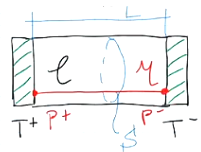
\includegraphics[width=0.4\linewidth]{conduttore_cilindrico}
\end{figure}
Si consideri un cilindro di materiale con due elettrodi, una sezione $S$ e una lunghezza 
$L$, una resistività $\eta$ assegnata e costante in $C$.
Si calcola la tensione $v$ tra i terminali considerando una linea retta tra essi
$$
v = \int_{p^+}^{p^-} \vec{E}\cdot\hat{t}dl = \int_{p^+}^{p^-} \eta\vec{J}\cdot\hat{t}dl
$$
Ricordando però che $\sqrt{S} << L \Rightarrow \vec{J} = \frac{i}{S}\hat{t}$ sostituendo
$$
v = \int_{p^+}^{p^-} \eta\frac{i}{S}dl \stackrel{(1)}{=} \eta\frac{i}{S} L = \eta\frac{L}{S}i = R\cdot i
$$
Il passaggio $(1)$ è valido se la sezione del cilindro è costante, con $R=\eta\frac{L}{S}$ 
detta anche seconda legge di Ohm.

\newpage
\subsection{Valutazione della resistenza di terra}
Si considerino due elettrodi sferici concentrici di raggio $a$ e $b$, ai quali colleghiamo 
un generatore che sostiene la tensione $v$ come in figura
\begin{figure}[H]
\centering
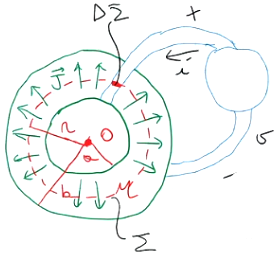
\includegraphics[width = 0.4\linewidth]{resistenza_terra}
\end{figure}
Si può determinare la corrente $i$ uscente dal generatore se supponiamo che tra i due mezzi
esista un elemento di resistività $\eta$, ci sarà un campo elettrico e di densità di 
corrente radiale dovuto alla 
distribuzione di carica positiva sull'elettrodo interno e negativa su quello esterno.
Utilizzando il metodo volt-amperometrico si ricava la resistenza del materiale
$$
R = \frac{v}{i}
$$
Si considera una superficie sferica di centro $O$ e raggio $r$ si applica ancora una volta
il principio di conservazione della carica alla superficie $\Sigma$ ottenuta
$$
\oiint_\Sigma \vec{J}\cdot\hat{n}dS = 0
$$
Per ragioni di simmetria sferica la densità di corrente ha la sola componente radiale
$\vec{J} = J_r(r)$ è quindi un problema monodimensionale.
$$
\iint_{\Sigma -\Delta\Sigma} \vec{J}\cdot\hat{n}dS + \iint_{\Delta\Sigma} \vec{J}
\cdot\hat{n}dS = 0
$$
il contributo che attraversa la superficie $\Delta\Sigma$ è $-i$ mentre l'area
dell'altra superficie si può approssimare alla superficie sferica di raggio $r$ con area
pari a $4\pi r^2$.
$$
4\pi r^2 J_r(r) - i = 0 \Rightarrow J_r(r) = \frac{i}{4\pi r^2}
$$
Il campo sarà dunque
$$
\vec{E} = \eta\vec{J} = \frac{\eta}{4\pi r^2} i
$$
\newpage
La tensione tra due punti posti sugli elettrodi sarà
$$
v = V(P_1) - V(P_2) = \int_{P_1}^{P_2} \vec{E}\cdot\hat{t}dl = \int_{r_1}^{r_2}
\eta\frac{i}{4\pi r^2} dr = \eta \frac{i}{4\pi} \left[-\frac{1}{r}\right]_a^b  = 
$$
$$
= \frac{\eta}{4\pi}\left(\frac{1}{a} -\frac{1}{b}\right) i \Rightarrow R = \frac{v}{i} = 
\frac{\eta}{4\pi}\left(\frac{1}{a} - \frac{1}{b}\right)
$$
La resistenza di terra si ottiene facendo tendere il raggio del dispersore esterno $(b)$
all'infinito come se fosse un piano, la formula per calcolare la resistenza di terra
dipende solo dal raggio del dispersore $a$ e dalla resistività del suolo
$$
R_T = \frac{\eta}{4\pi}\frac{1}{a}
$$

\subparagraph{Dispersore emisferico}
Si collega un dispersore emisferico interrato nel piano di terra, si collega un
generatore di tensione ad un punto del dispersore e un punto abbastanza
distante nel piano di terra.
\begin{figure}[H]
\centering
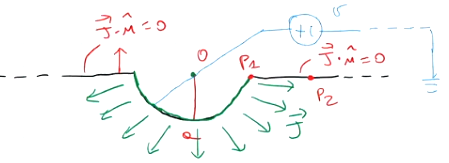
\includegraphics[width = 0.4\linewidth]{dispersore_emisferico}
\end{figure}
Analizzando le condizioni al contorno del suolo
$$
\vec{J}\cdot\hat{n} = 0
$$
la densità di corrente sarà dunque ancora radiale rispetto al dispersore,
mantenendo il vantaggio matematico della simmetria $(\vec{J} = J_r(r))$
la superficie sarà però la metà della sfera e di conseguenza 
$$
J_r(r) = \frac{i}{2\pi r^2}
$$
Presa dunque una linea che congiunge un punto tangente al dispersore e un punto a
sufficiente distanza si può calcolare la tensione
$$
V(P_1) - V(P_2) = \int_{P_1}^{P_2} \vec{E}\cdot\hat{t} dl = -\int_{r_1}^{r_2} \eta\frac{i}{2\pi r^2} dr = \frac{\eta}{2\pi} \left[-\frac{1}{r}\right]_a^{r_2}\cdot i
$$
$$
V(P_1)-V(P_2) = \frac{\eta}{2\pi}\left(\frac{1}{a}-\frac{1}{r_2}\right) i
$$
La normativa specifica il limite massimo della \textit{tensione di passo}
ossia la tensione presente a distanza di un metro (un passo) $V(r) - V(r+1)$
$$
\frac{\eta}{2\pi}\left(\frac{1}{r} - \frac{1}{r+1}\right) i = \frac{\eta}{2\pi}\left(\frac{r+1 - r}{r^2 + r}\right) i = \frac{\eta}{2\pi}\left(\frac{1}{r^2+r}\right) i
$$
L'andamento della tensione di passo è del tipo $\frac{1}{r^2}$, per questo motivo è 
necessario prevedere una zona di sicurezza nell'intorno del dispersore non calpestabile.

\subsection{Bilancio energetico in un circuito elementare}
Preso un circuito con due componenti collegati, un generatore ed un utilizzatore $C_1$ e 
$C_2$ collegati mediante gli elettrodi $T^+$ e $T^-$, si orientano le regioni dei 
terminali. 
\begin{figure}[H]
\centering
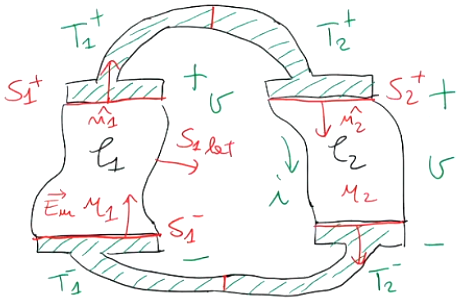
\includegraphics[width=0.6\linewidth]{generatore_utilizzatore}
\end{figure}
Si considerano le regioni dei terminali conduttori ideali
$$
\begin{aligned}
T_1^+ \cup T_2^+ &\qquad \vec{E} = 0,\ \vec{J} \neq 0\\
T_1^- \cup T_2^- &\qquad \vec{E} = 0,\ \vec{J} \neq 0
\end{aligned}
$$
mentre le regioni dei conduttori saranno caratterizzate dalle seguenti espressioni
$$
\begin{aligned}
\vec{J} &= \gamma_1 (\vec{E}+\vec{E_m}) \qquad &\text{in } C_1\\
\vec{J} &= \gamma_2\vec{E} \qquad &\text{in } C_2
\end{aligned}
$$
La potenza necessaria a muovere le cariche nel circuito è misurabile con l'integrale del lavoro per unità di tempo e per unità di carica nel volume
$$
P^{(a)}_{C_1} = \iiint_{C_1} \vec{E}\cdot\vec{J} dV = \iiint_{C_1} \left(\eta_1\vec{J} - 
\vec{E}_m\right)\cdot\vec{J} dV = \iiint_{C_1} \eta_1 |\vec{J}|^2dV - \iiint_{C_1} \vec{E}_m\cdot\vec{J}dV
$$
Il primo termine sicuramente maggiore di zero è la dissipazione per effetto Joule
della resistenza interna del generatore. Il secondo termine (negativo) è l'energia 
assorbita dal generatore, il segno opposto indica che è erogata.

Ricordando che $nabla\cdot(f\vec{v}) = f\nabla \cdot\vec{v} + \nabla f \cdot\vec{v}$ e che
nelle ipotesi di conduzione stazionaria $\vec{E} = -\nabla V $ e $\nabla\cdot\vec{J}= 0$

allora
$$
\nabla\cdot(V\vec{J}) = \cancel{V\nabla\cdot\vec{J}} + \nabla V \cdot \vec{J} = -\vec{E}\cdot\vec{J}
$$
sostituendo nell'integrale
$$
\iiint_{C_1} - \nabla\cdot(V\vec{J}) dV \stackrel{\text{T. divergenza}}{=} \iint_{\partial C_1} - V\vec{J}\cdot\hat{n}dS = \iint_{S_1^+}-V_1^+\vec{J}\cdot\hat{n}_1dS - \iint_{S_1^-}-V_1^-\vec{J}\cdot\hat{n}_1dS
$$
$$
-V_1^+ i + V_1^-i = -(V_1^+-V_1^-)\cdot i = - v\cdot i = \iiint_{C_1} \eta_1 |\vec{J}|^2dV - \iiint_{C_1} \vec{E}_m\cdot\vec{J}dV
$$
che è proprio la potenza assorbita dal generatore.

Si calcola ora la potenza assorbita dal carico $(C_2)$
$$
P_{C_2}^{(a)} = \iiint_{C_2} \vec{E}\cdot\vec{J} dV = \iiint_{C_2} \eta_2 |\vec{J}|^2 dV = v\cdot i
$$
utilizzando la stessa identità vettoriale, in conclusione
$$
P_{C_1}^{(e)} = -P_{C_1}^{(a)} =  \iiint_{C_1} \vec{E}_m\cdot\vec{J}dV - \iiint_{C_1} \eta_1 |\vec{J}|^2dV = v\cdot i = \iiint_{C_2} \eta_2 |\vec{J}|^2 dV = P_{C_2}^{(a)}
$$
ossia si è dimostrato mediante la formulazione campistica che la potenza erogata
dal generatore è pari a quella assorbita dal resistore.
Il modello circuitale equivalente è pari a quello del generatore reale con resistenza
interna $R_i$ collegato al carico $R$.
$$
P_{gen}^{(e)} = v\cdot i = (E_0 -R_i i ) = E_0 i - R_i i^2 = P_R^{(a)} = Ri^2
$$
